\section{Introduction}
\label{sec:introduction}

The Transmission Control Protcol, short TCP, is most popular communication
protcol on the Internet. To make it scaleable and adaptive to the current
condition of network without overloading it, congestion control mechanism are
used. Part of these algorithm is TCP slow start as decribed in
RFC5681~\cite{rfc5681}.

The TCP slow algoritm limits the number of bytes it sends on a new tcp
connection before waiting for an acknowledgement. On every acknowleged packet
the sender increases the window size by one segment until the Slow-start
threshold (\emph{ssthres}) is reached  or the receiver advertises a lower
receiver window (\emph{rwnd}) in its tcp header. The exponential grow of the
window every roundtrip will be also stopped if TCP detects packet loss. This
could be indicated by either a duplicate acknowlegdment of the receiver or a
timeout. Depending on the congestion algorithm in use the sender will then
behave differently. TCP Reno~\cite{rfc2581} is currently the most widely
deployed. On timeout it will reduce the congestion window to 1. If it receives
an acknowledgment for the same packet three times in a row, it will half
congestion window. The new Slow-Start threshold will be set to the
current window. The sender assumes that the packet after the one, it received
duplicate ACKs for, got lost and will perform a retransmit (also known as Fast
Retransmit). It then enters a phase called Fast Recovery. In this phase the
sender will increase the congestion window only one segment per round trip,
which is equivalent to linear growth.

Other congestion algorithm have slightly different behavior on how they behave
when congestion is detected. In picture~\ref{fig:cwnd_tcp_algos} the grow of tcp
congestion windows for different tcp congestion algorithm is depicted. An
Assumption that most tcp congestion algorithm make is that the majority packet
loss in the network occurs because overloading the network at bottlenecks rather
thank faulty transmission. Router in the network have a limited queue they fill
up before they begin to drop IP packets. Bottlenecks in the network occur
because links have assymmetric bandwith or usage.

\begin{figure*}[ht]
\footnotesize
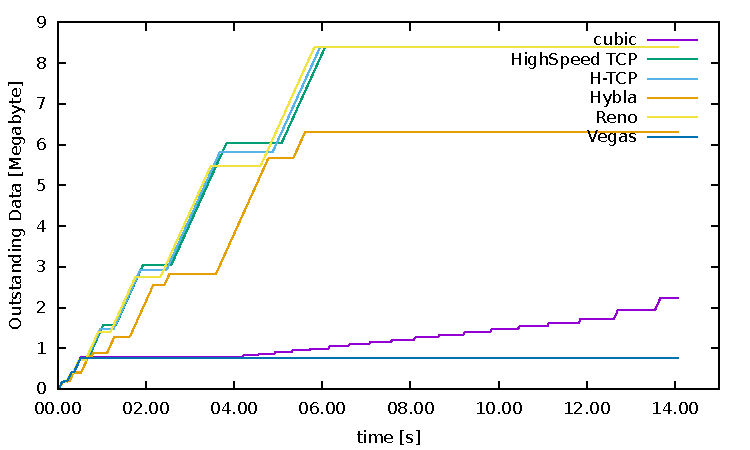
\includegraphics[scale=0.8]{figure/b2a_owin.pdf}
\caption{Congestion window grow over time for different tcp congestion
algorithm for a single connection over 10mbit link with a forwarding delay of
10ms}
\label{fig:cwnd_tcp_algos}
\end{figure*}

The initial congestion window therefor defines the upper limit of bytes a sender assumes at
the beginning.
